\documentclass{article}

\usepackage{fullpage}
\usepackage{hyperref}
\marginparwidth 0pt
\oddsidemargin 0pt
\evensidemargin 0pt
\topmargin 0pt
\textwidth 16cm
\textheight 21cm

\usepackage{Sweave}

\begin{document}

\Sconcordance{concordance:QTL_Mapping_DO_Mice.tex:QTL_Mapping_DO_Mice.Rnw:%
1 90 1 1 2 1 0 3 1 3 0 1 2 6 1 1 2 4 0 1 2 2 1 1 2 1 0 1 1 3 0 1 2 2 1 %
1 2 4 0 1 2 2 1 1 3 8 0 1 2 2 1 1 3 2 0 1 1 3 0 1 2 2 1 1 2 4 0 1 2 2 1 %
1 -4 1 8 6 1 1 2 4 0 1 2 2 1 1 -4 1 8 10 1 1 2 1 0 1 1 9 0 1 2 4 1 1 4 %
12 0 2 1 7 0 1 2 2 1 1 -6 7 0 1 2 5 0 1 8 6 1 1 3 2 0 1 1 5 0 1 1 33 0 %
1 2 3 1}

\setkeys{Gin}{width=1.0\textwidth}

\title{QTL Mapping using Diversity Outbred Mice}
\author{Daniel M. Gatti}
\date{08 October 2013}
\maketitle

\section{Introduction}

Quantitative Trait Locus (QTL) mapping in DO mice is performed in several steps. First, we use the founder haplotype contributions to perform linkage mapping. In the mapping model, we adjust for kinship between DO mice using the R package \href{http://cran.r-project.org/web/packages/QTLRel/}{QTLRel}. Then, we perform permutations to determine and empirical signficance threshold. Next, we select chromosomes with QTL peaks above the signficance threshold, examine the founder allele effects and determine support intervals. Finally, we impute the founder SNPs onto the DO genomes to perform association mapping in the QTL intervals.
  
\section{Mapping Models}

\subsection{Linkage Mapping}
  
Linkage mapping involves the use of founder haplotype probabilities. We perform point mapping at each marker on the array. We fit an additive model that regresses the phenotype on the eight founder haplotype contributions and incorporates an adjustment for the kinship between samples. 
  
\begin{equation}
y = X\alpha + H\beta + Zu + \varepsilon
\end{equation}

where:

\begin{itemize}
  \item{\textit{n} is the number of samples}
  \item{\textit{y} is an \textit{n} x 1 vector of phenotype values for each sample}
  \item{\textit{X} is an \textit{n} x \textit{p} matrix of \textit{p} fixed covariates (sex, diet, etc.) }
  \item{$\alpha$ is a \textit{p} x 1 vector of fixed effects }
  \item{\textit{H} is an \textit{n} x 8 matrix of founder haplotype contributions (each row sums to 1) }
  \item{$\beta$ is an 8 x 1 vector of founder haplotype effects }
  \item{\textit{Z} is an \textit{n} x \textit{n} matrix of error covariances between samples }
  \item{\textit{u} is an \textit{n} x 1 vector of ???}
  \item{$\varepsilon$ is an \textit{n} x 1 vector of residual errors}
\end{itemize}

\subsection{Association Mapping}

Between each pair of markers, we assign the genotype state with the highest probability to each DO sample. We then query the \href{ftp://ftp.jax.org/SNPtools/variants/}{Sanger Mouse Genomes SNP file} to obtain all of the founder SNPs in the interval.

For each Sanger SNP, we impute the Sanger SNPs onto DO genomes as follows:

\begin{equation}
a_{j}=\sum_{i=1}^{8}s_{i}h_{ij}
\end{equation}

where:

\begin{itemize}
  \item{\texit{a} is the allele call (coded as 0, 1 or 2) for sample \textit{j} }
  \item{\texit{s} is the Sanger founder allele call (coded as 0 or 1) }
  \item{\texit{h} is the founder haplotype contribution of founder \textit{i} for sample \textit{j} }
\end{itemize}

\begin{equation}
y = X\alpha + A\beta + Zu + \varepsilon
\end{equation}

where:

\begin{itemize}
  \item{\textit{n} is the number of samples}
  \item{\textit{y} is an \textit{n} x 1 vector of phenotype values for each sample}
  \item{\textit{X} is an \textit{n} x \textit{p} matrix of \textit{p} fixed covariates (sex, diet, etc.) }
  \item{$\alpha$ is a \textit{p} x 1 vector of fixed effects }
  \item{\textit{A} is an \textit{n} x 3 matrix of imputed allele calls }
  \item{$\beta$ is an 3 x 1 vector of allele effects }
  \item{\textit{Z} is an \textit{n} x \textit{n} matrix of error covariances between samples }
  \item{\textit{u} is an \textit{n} x 1 vector of ???}
  \item{$\varepsilon$ is an \textit{n} x 1 vector of residual errors}
\end{itemize}

\section{QTL Mapping}

We will use example data from Svenson et.al, \href{http://www.ncbi.nlm.nih.gov/pubmed/22345611}{\textit{Genetics}, 2012}. Breifly, 149 mice (75 F, 74 M) were placed on either a chow (n = 100) or a high fat diet (n = 49). A  variety of clinical phenotypes were measured at two time points, roughly 14 weeks apart.  In this example, we will map the hemoglobin distribution width (HDW) at the second time point.

\begin{Schunk}
\begin{Sinput}
> library(DOQTL)
> library(MUGAExampleData)
> data(pheno)
> data(model.probs)
\end{Sinput}
\end{Schunk}

QTL mapping requires phenotype and genotype data. Here, we have a \texttt{data.frame} of phenotypes called \texttt{pheno} and a 3D array of founder haplotype contributions (num.samples x 8 founders x num.markers) called \texttt{model.probs}. The sample IDs must be in rownames(pheno) and dimnames(model.probs)[[1]] and they must match each other. We will map the hemoglobin distribution width at time point 2 (HDW2).

\vspace{5 mm}

First, we need to create a kinship matrix using the founder contributions.

\begin{Schunk}
\begin{Sinput}
> K = kinship.probs(model.probs)
\end{Sinput}
\end{Schunk}

Second, we need to create a matrix of additive covariates to run in the model. In this case, we will use sex, diet and CHOL1. Note that the sample IDs must be in \texttt{rownames(covar)}.

\begin{Schunk}
\begin{Sinput}
> covar = data.frame(sex = as.numeric(pheno$Sex == "M"), diet = as.numeric(pheno$Diet == "hf"))
> rownames(covar) = rownames(pheno)
\end{Sinput}
\end{Schunk}

Third, we need to get the marker locations on the array.

\begin{Schunk}
\begin{Sinput}
> load(url("ftp://ftp.jax.org/MUGA/MM_snps.Rdata"))
\end{Sinput}
\end{Schunk}

Fourth, we map the phenotype using \texttt{scanone}.

\begin{Schunk}
\begin{Sinput}
> qtl = scanone(pheno = pheno, pheno.col = "HDW2", probs = model.probs, K = K,
+               addcovar = covar, snps = MM_snps)
\end{Sinput}
\begin{Soutput}
[1] "HDW2"
\end{Soutput}
\end{Schunk}

Fifth, we run permutations to determine significane thresholds. We recommend running at least 1,000 permutations. In this demo, we run 100 permutations to save time.

\begin{Schunk}
\begin{Sinput}
> perms = scanone.perm(pheno = pheno, pheno.col = "HDW2", probs = model.probs, 
+         K = K, addcovar = covar, snps = MM_snps, nperm = 100)
> thr = quantile(perms, probs = 0.95)
\end{Sinput}
\end{Schunk}

We then plot the LOD curve for the QTL.

\begin{Schunk}
\begin{Sinput}
> qtl.plot(qtl, sig.thr = thr, main = "HDW2")
\end{Sinput}
\end{Schunk}

\begin{figure}
\begin{center}
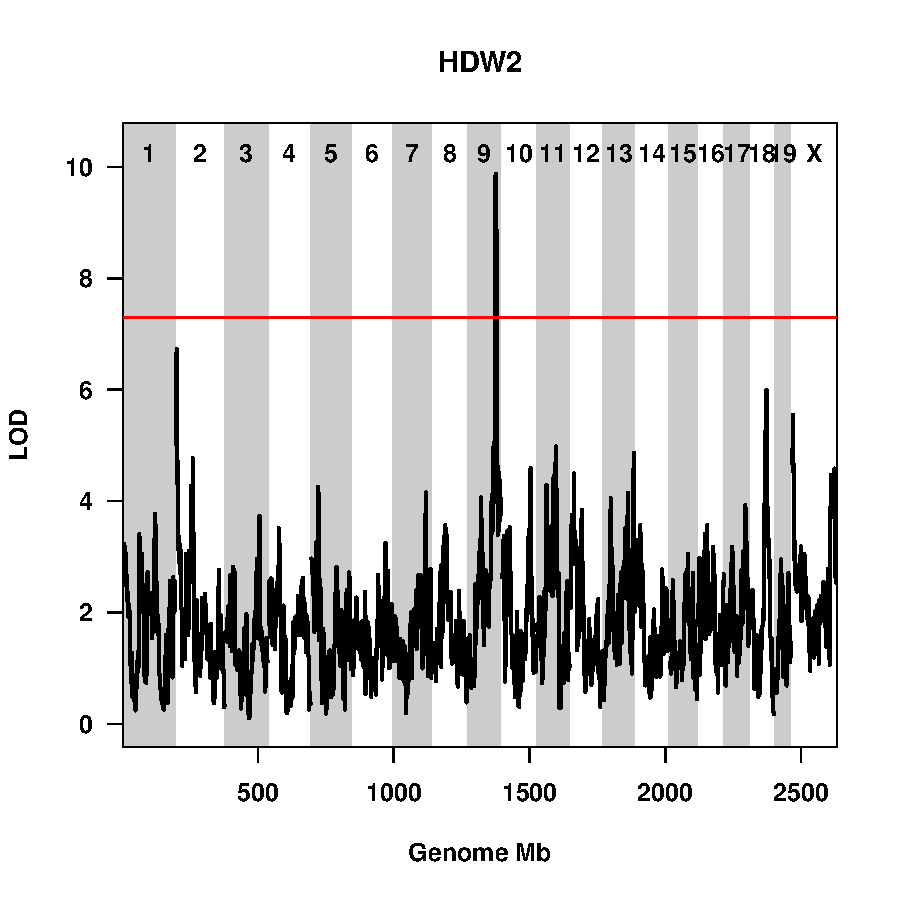
\includegraphics{QTL_Mapping_DO_Mice-fig1}
\end{center}
\caption{QTL plot of HDW2. The LOD of the mode in Eqn. 1 is plotted along the mouse genome. The red line is the p $<$ 0.05 significance threshold.}
\label{fig:qtlplot}
\end{figure}

The largest peak appears on Chr 9. The linkage mapping model (Eqn. 1) produces an estimate of the effect of each founder allele at each marker. We can plot these effects (model coefficients) on Chr 9 to see which founders contribute to a high HDW.

\begin{Schunk}
\begin{Sinput}
> coef.plot(qtl, chr = 9)
\end{Sinput}
\end{Schunk}

\begin{figure}
\begin{center}
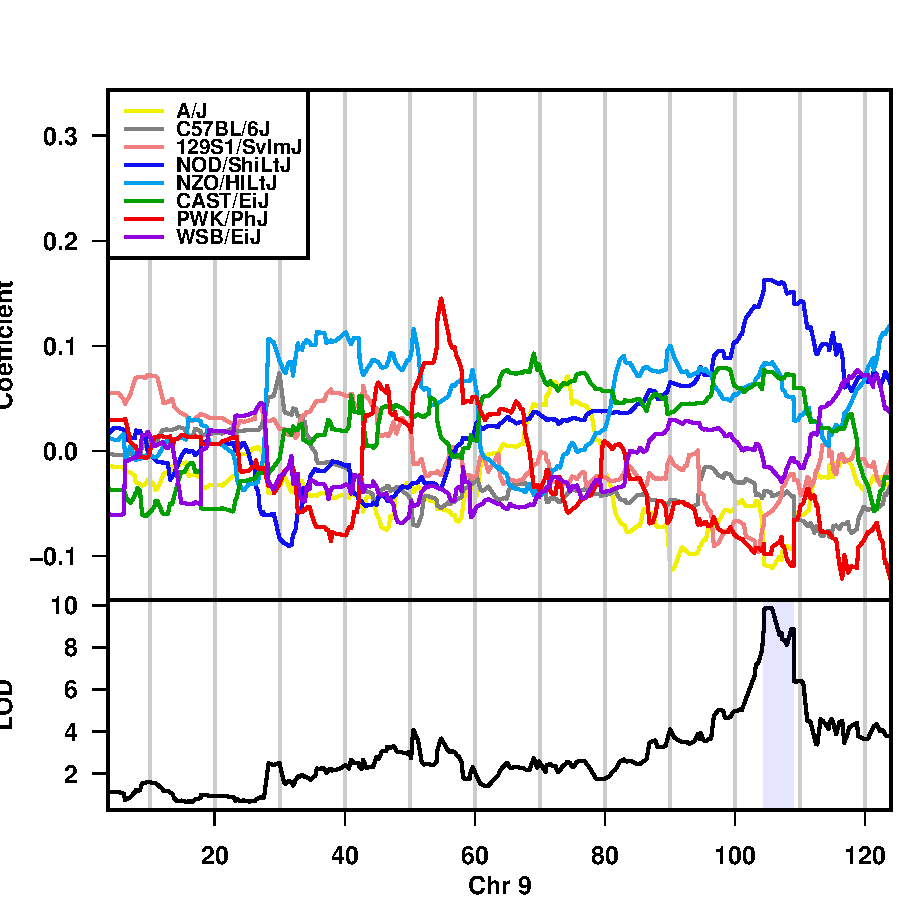
\includegraphics{QTL_Mapping_DO_Mice-fig2}
\end{center}
\caption{Coefficient plot of HDW2 on Chr 9. The top panel shows the 8 estimated founder allele effects along Chr 9. The NOD/ShiLtJ allele contributes to high values and the A/J and PWK/PhJ alleles contribute to low values. The bottom panel shows the LOD score.}
\label{fig:qtlplot}
\end{figure}

Note that the DO mice with alleles from three strains, 129S1/SvImJ, NZO/HlLtJ and WSB/EiJ,
have lower changes in cholesterol than the other five strains. Remember
these strains because they will appear again below.
\vspace{5 mm}  
We then determine the width of the QTL support interval using \texttt{bayesint}. Note that this function only provides reasonable support intervals if there is a single QTL on the chromosome.

\begin{Schunk}
\begin{Sinput}
> interval = bayesint(qtl, chr = 9)
> interval
\end{Sinput}
\begin{Soutput}
            SNP_ID Chr Mb_NCBI38      cM perc.var      lrs      lod
1             <NA>   9  104.2953 56.6120 0.250206 38.90393 8.447880
40682 UNC091160886   9  105.5128 56.7432 0.286097 45.49603 9.879338
3             <NA>   9  108.9904 59.6310 0.251963 39.24904 8.522820
\end{Soutput}
\end{Schunk}

The QTL support interval is 4.7 Mb wide.
\vspace{5 mm}
Finally, we narrow the candidate gene list by imputing the founder SNPs onto the DO genomes. This idea is essentially \href{http://www.ncbi.nlm.nih.gov/pubmed/22847376}{assocation mapping} in an outbred population.

\begin{Schunk}
\begin{Sinput}
> ma = merge.analysis(pheno = pheno, pheno.col = "HDW2", probs = model.probs, K = K,
+                     addcovar = covar, snps = MM_snps, chr = interval[1,2], 
+                     start = interval[1,3], end = interval[3,3])
\end{Sinput}
\begin{Soutput}
[1] "Mapping with 135 samples."
[1] "Retrieving SNPs..."
[1] "Retrieved 67113 SNPs."
[1] "Finding unique SNP patterns..."
[1] "Calculating LOD"
\end{Soutput}
\begin{Sinput}
> tmp = merge.plot(ma, thr = 4)
> unique(tmp$sdps)
\end{Sinput}
\begin{Soutput}
[1] 00010000 00010100 00111100 00011000
79 Levels: 00000001 00000010 00000011 00000100 00000101 00000110 ... 10111111
\end{Soutput}
\end{Schunk}

\begin{figure}
\begin{center}
\begin{Schunk}
\begin{Soutput}
[1] "Mapping with 135 samples."
[1] "Retrieving SNPs..."
[1] "Retrieved 67113 SNPs."
[1] "Finding unique SNP patterns..."
[1] "Calculating LOD"
\end{Soutput}
\begin{Soutput}
[1] 00010000 00010100 00111100 00011000
79 Levels: 00000001 00000010 00000011 00000100 00000101 00000110 ... 10111111
\end{Soutput}
\end{Schunk}
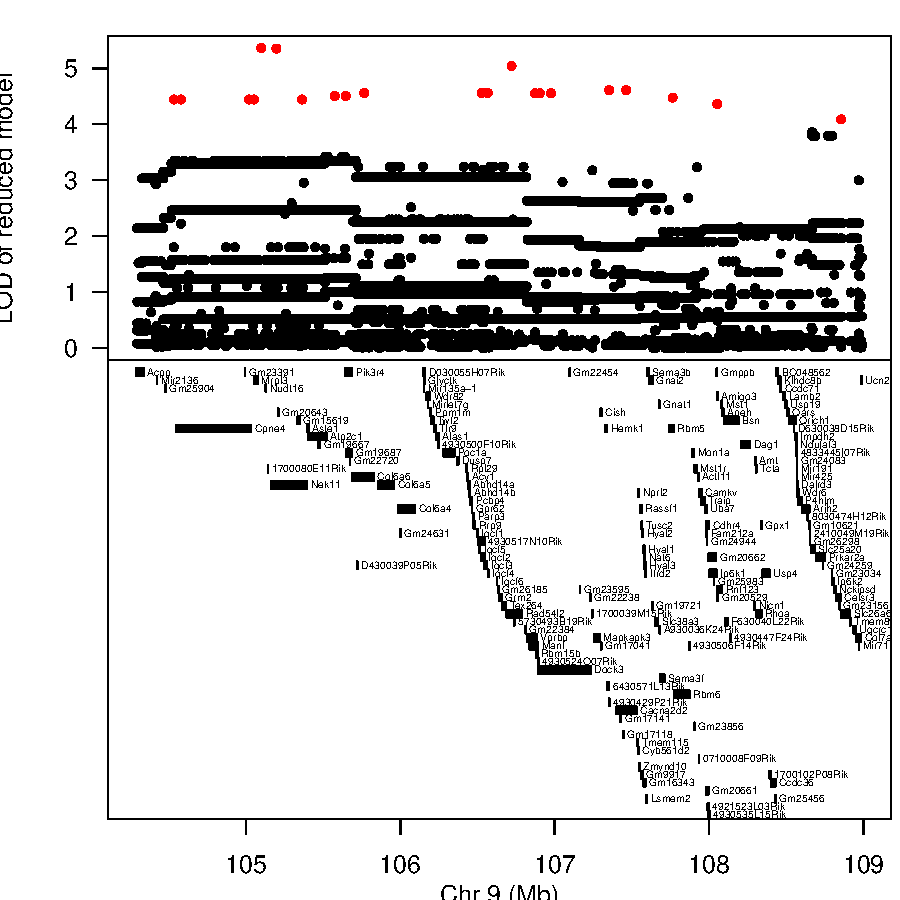
\includegraphics{QTL_Mapping_DO_Mice-fig3}
\end{center}
\caption{Association mapping plot of HDW2 in the Chr 9 support interval. The top panel shows the LOD score from assocation mapping (Eqn. 3) in the QTL support interval. The bottom panel shows the genes and non-coding RNAs from the \href{http://informatics.jax.org/}{Mouse Genome Informatics} database.}
\label{fig:qtlplot}
\end{figure}

We can get the genes in the QTL interval using the \texttt{get.mgi.features()} function.

\begin{Schunk}
\begin{Sinput}
> mgi = get.mgi.features(chr = interval[1,2], start = interval[1,3],
+       end = interval[3,3], type = "gene", source = "MGI")
> nrow(mgi)
\end{Sinput}
\begin{Soutput}
[1] 169
\end{Soutput}
\begin{Sinput}
> head(mgi)
\end{Sinput}
\begin{Soutput}
    seqid source type     start      stop score strand phase              ID
1       9    MGI gene 104288240 104337728     .      -     . MGI:MGI:1928480
191     9    MGI gene 104426113 104426187     .      +     . MGI:MGI:4358922
198     9    MGI gene 104481368 104481510     .      -     . MGI:MGI:5455681
202     9    MGI gene 104547286 105034544     .      +     . MGI:MGI:1921270
361     9    MGI gene 104994916 104995019     .      +     . MGI:MGI:5453168
435     9    MGI gene 105053239 105077476     .      +     . MGI:MGI:2137204
       Name Parent
1      Acpp     NA
191 Mir2136     NA
198 Gm25904     NA
202   Cpne4     NA
361 Gm23391     NA
435   Mrpl3     NA
                                                                Dbxref
1   VEGA:OTTMUSG00000024988,NCBI_Gene:56318,ENSEMBL:ENSMUSG00000032561
191                     NCBI_Gene:100316725,ENSEMBL:ENSMUSG00000089406
198                                         ENSEMBL:ENSMUSG00000089116
202 VEGA:OTTMUSG00000023466,NCBI_Gene:74020,ENSEMBL:ENSMUSG00000032564
361                                         ENSEMBL:ENSMUSG00000088204
435 VEGA:OTTMUSG00000023521,NCBI_Gene:94062,ENSEMBL:ENSMUSG00000032563
                               mgiName               bioType
1         acid phosphatase%2c prostate protein coding gene\r
191                      microRNA 2136          miRNA gene\r
198            predicted gene%2c 25904         snoRNA gene\r
202                          copine IV protein coding gene\r
361            predicted gene%2c 23391          miRNA gene\r
435 mitochondrial ribosomal protein L3 protein coding gene\r
\end{Soutput}
\end{Schunk}

There are 169 genes in the QTL support interval. Several SNPs have LOD scores above 4. This is a somewhat arbitrary cutoff and an appropriate threshold will be supplied in future version of DOQTL. In this case, there may be more than one variant that influences the phenotype.

\end{document}
